\documentclass{article}

\usepackage[utf8]{vietnam}
\usepackage{graphicx}
\usepackage{setspace}
\usepackage{fancyhdr}
\usepackage{pifont}

\usepackage{tikz}
\usetikzlibrary{calc}

\usepackage[left=3.5cm,right=2cm,top=2cm,bottom=2cm]{geometry}

\usepackage{listings}
\usepackage{xcolor}

\definecolor{dkgreen}{rgb}{0,0.6,0}
\definecolor{gray}{rgb}{0.5,0.5,0.5}
\definecolor{mauve}{rgb}{0.58,0,0.82}

\lstset{frame=tb,
    language=Java,
    aboveskip=3mm,
    belowskip=3mm,
    showstringspaces=false,
    columns=flexible,
    numbers=left,
    numberstyle=\small\color{gray},
    keywordstyle=\color{blue},
    commentstyle=\color{dkgreen},
    stringstyle=\color{mauve},
    breaklines=true,
    breakatwhitespace=true,
    tabsize=3
}

\usepackage[none]{hyphenat}
\tolerance=9999
\emergencystretch=10pt
\hyphenpenalty=10000
\exhyphenpenalty=100

\newcommand\para{\paragraph{} \hspace{0pt} \fontsize{13}{13}\selectfont \fontseries{b}\selectfont \indent}
\newcommand\subpara{\fontsize{13}{13}\selectfont \fontseries{b}\selectfont}
\newcommand\head{\fontsize{30}{20}\selectfont \fontseries{b}\selectfont}

\makeatletter
\renewcommand{\tableofcontents}{%
	\@starttoc{toc}%
}
\makeatother

\begin{document}
    \begin{tikzpicture}[overlay,remember picture]
    \draw [line width=2pt]
        ($ (current page.north west) + (3.0cm,-2.0cm) $)
        rectangle
        ($ (current page.south east) + (-2.0cm,2.5cm) $);
    \draw [line width=0.5pt]
        ($ (current page.north west) + (3.1cm,-2.1cm) $)
        rectangle
        ($ (current page.south east) + (-2.1cm,2.6cm) $);
    \end{tikzpicture}

	\begin{center}
		\pagenumbering{gobble}
		\fontsize{14}{20}\selectfont
		\textbf{ĐẠI HỌC QUỐC GIA HÀ NỘI\\
			\textbf{TRƯỜNG ĐẠI HỌC KHOA HỌC TỰ NHIÊN\\}
			\textbf{KHOA TOÁN - CƠ - TIN HỌC}}
		\vspace{0.8cm}
		\begin{figure}[htp]
			\begin{center}
				
\includegraphics[scale=0.5]{./image/logohus.png}
			\end{center}
		\end{figure}
		\fontsize{16}{20}\selectfont\textbf{BÁO CÁO CUỐI KỲ\\}
		\fontsize{20}{20}\selectfont\textbf{CÁC THÀNH PHẦN PHẦN MỀM\\}
	\vspace{1cm}
		\setstretch{1.5}
	    \fontsize{18}{18}\selectfont\textbf{Tên Đề Tài: DESIGN PATTERNS}
\textit{(nhóm 1)\\}
	    \vspace{1cm}
	 \end{center}

    \begin{flushleft}
		\fontsize{16}{20}\selectfont
		\textit{Sinh viên thực hiện:}\\
		\textbf{Phạm Bá Thắng - 20001976}\\
		\textbf{La Thị Anh Thư - 20001980}\\
    \end{flushleft}
	\vspace{3cm}
    \begin{center}
		\fontsize{14}{20}\selectfont
		\textbf{HÀ NỘI, 1/2022}
	\end{center}
	\pagebreak

	\pagestyle{fancy}
	\fancyhf{}
	\chead{\thepage}
	\renewcommand{\headrulewidth}{0pt}
	\begin{center}
		\head{LỜI CẢM ƠN}
		\hspace{15pt}
	\end{center}
	    \para{Đầu tiên, chúng em xin gửi lời cảm ơn chân thành đến Trường Đại học Khoa học Tự nhiên đã đưa môn học Các thành phần phần mềm vào chương trình giảng dạy. Đặc biệt, chúng em xin gửi lời cảm ơn sâu sắc đến giảng viên bộ môn - Thầy Quản Thái Hà đã dạy dỗ, truyền đạt những kiến thức quý báu cho chúng em trong suốt thời gian học tập vừa qua. Trong thời gian tham gia lớp học Các thành phần phần mềm của thầy, chúng em đã có thêm cho mình nhiều kiến thức bổ ích, tinh thần học tập hiệu quả, nghiêm túc. Đây chắc chắn sẽ là hành trang để chúng em có thể vững bước sau này.}
	    \para{Bộ môn Các thành phần phần mềm là môn học thú vị, vô cùng bổ ích và có tính thực tế cao. Đảm bảo cung cấp đủ kiến thức, gắn liền với nhu cầu phát triển của sinh viên. Tuy nhiên, khả năng tiếp nhận kiến thức của mỗi người luôn tồn tại những hạn chế nhất định. Do đó, bài báo cáo khó có thể tránh khỏi những thiếu sót. Kính mong thầy xem xét và góp ý để bài báo cáo của chúng em được hoàn thiện hơn.}
	    \para{Kính chúc thầy sức khỏe, hạnh phúc, thành công trên con đường sự nghiệp giảng dạy.}
	\pagebreak


	\begin{center}
		\head{Mục Lục}
	\end{center}
	\setstretch{1.5}
	\fontsize{13}{13}\selectfont
	\tableofcontents
\pagebreak


	\pagenumbering{arabic}\setcounter{page}{1}
	\begin{center}
		\fontsize{30}{20}\selectfont \part{Tóm tắt}
	\end{center}
	    \para{Design pattern là các giải pháp tổng thể đã được tối ưu hóa, được tái sử dụng cho các vấn đề phổ biến trong thiết kế phần mềm mà chúng ta thường gặp phải hàng ngày. Đây là tập các giải pháp đã được suy nghĩ, đã giải quyết trong tình huống cụ thể.}
	    \para{Design pattern có thể thực hiện được ở phần lớn các ngôn ngữ lập trình. Nó giúp bạn giải quyết vấn đề một cách tối ưu nhất, cung cấp cho bạn các giải pháp trong lập trình hướng đối tượng (OOP).}
	    \para{Design pattern gồm 23 loại được chia thành 3 nhóm:}

	    \begin{itemize}
	        \item[-]\subpara{Creational Pattern (nhóm khởi tạo) gồm: Factory Method, Abstract Factory, Builder, Prototype, Singleton. Những Design pattern loại này cung cấp một giải pháp để tạo ra các object và che giấu được logic của việc tạo ra nó, thay vì tạo ra object một cách trực tiếp bằng cách sử dụng method new. Điều này giúp cho chương trình trở nên mềm dẻo hơn trong việc quyết định object nào cần được tạo ra trong những tình huống được đưa ra}
	        \item[-]\subpara{Structural Pattern (nhóm cấu trúc) gồm: Adapter, Bridge, Composite, Decorator, Facade, Flyweight và Proxy. Những Design pattern loại này liên quan tới class và các thành phần của object. Nó dùng để thiết lập, định nghĩa quan hệ giữa các đối tượng.}
	        \item[-]\subpara{Behavioral Pattern (nhóm hành vi) gồm: Interpreter, Template Method, Chain of Responsibility, Command, Iterator, Mediator, Memento, Observer, State, Strategy và Visitor. Nhóm này dùng trong thực hiện các hành vi của đối tượng, sự giao tiếp giữa các object với nhau.}
	    \end{itemize}
    \pagebreak
		\begin{center}
		    \hspace{0pt}
            \vfill
		    \fontsize{30}{20}\selectfont\part{Nhóm Khởi tạo - Creational Pattern}
		    \vfill
            \hspace{0pt}
	    \end{center}
	\pagebreak

		\section{Singleton}
        \subsection{Định Nghĩa Và Mô Hình Cấu Trúc}
        \begin{itemize}
            \item[-]\subpara{Singleton đảm bảo chỉ duy nhất một instance được tạo ra và cung cấp một method để có thể truy xuất được instance đó mọi lúc mọi nơi trong chương trình.}
            \item[-]\subpara{Singleton ẩn đi hàm dựng của class và sử dụng hàm các hàm có sẵn bên trong để tạo đối tượng}
        \end{itemize}
		\begin{figure}[htp]
			\begin{center}
				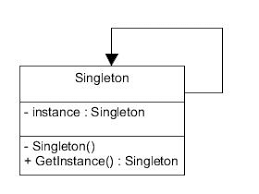
\includegraphics[scale=1]{./image/singleton-pattern.png}
			\end{center}
		\end{figure}

        \subsection{Đặc điểm}
        \begin{itemize}
            \item[-]\subpara{Đảm bảo rằng một lớp chỉ có một instance}
            \item[-]\subpara{Dễ dàng truy cập vào instance này}
            \item[-]\subpara{Kiểm soát việc khởi tạo nó}
            \item[-]\subpara{Giới hạn số lượng instance}
            \item[-]\subpara{Có thể truy cập như một biến toàn cục}
        \end{itemize}
		\subsection{Mục Đích Sử Dụng}
		\begin{itemize}
			\item[-]\subpara{Là dạng class nên có thể sử dụng với nhiều design pattern khác nhau}
			\item[-]\subpara{Sử dụng làm biến toàn cục với các ưu điểm như:}
			\begin{itemize}
			    \item[+]\subpara{Không làm rối loạn danh sách các biến toàn cục vì không tạo ra các biến không cần thiết}
			    \item[+]\subpara{Chúng cho phép phân bổ và khởi tạo khi cần (call-by-need), trong khi tạo nhiều các biến toàn cục ngay từ đầu sẽ luôn tiêu tốn tài nguyên.}
		    \end{itemize}
		    \item[-]\subpara{Ví dụ như dùng để ghi log rất thích hợp vì chúng ta chỉ cần 1 bản ghi log duy nhất cho mỗi phiên đồng thời lại cần ở tất cả các bộ phận của chương trình}
		\end{itemize}

		\subsection{Code khuôn mẫu}
		\begin{lstlisting}
    public class Singleton {
        private static final Singleton INSTANCE = new Singleton();
        private Singleton() {}
        public static Singleton getInstance(){
            if(INSTANCE == null){
                INSTANCE = new Singleton();
            }
            return INSTANCE;
        }
    }
        \end{lstlisting}

		\subsection{Giải thích Design Pattern}
		\begin{itemize}
		    \item[-]\subpara{Giải thích theo mô hình}
		    \begin{itemize}
			    \item[+]\subpara{Private constructor để hạn chế truy cập từ class bên ngoài.}
			    \item[+]\subpara{Đặt private static final variable đảm bảo biến chỉ được khởi tạo trong class và duy nhất 1 lần.}
		    \end{itemize}
		    \item[-]\subpara{Giải thích theo code khuôn mấu}
		    \begin{itemize}
			    \item[+]\subpara{Có một method public static để return instance được khởi tạo ở trên và một đoạn if để kiểm tra xem instance tồn tại chưa, nếu chưa sẽ gọi hàm khởi tạo. Hàm này được gọi là accessor.}
			    \item[+]\subpara{Sau đó là các hàm để sử dụng.}
			\end{itemize}
		\end{itemize}

		\subsection{Ví Dụ Sử Dụng Trong Thực Tế}
            \subpara{Simple Logger\\https://github.com/blaplafla13th/design-partterns/tree/main/src/singleton}
    \para{Tạo một logger theo Singleton pattern, sau đó chúng ta thêm các hàm kiểm tra file (check), hàm ghi file (write) và hàm đọc file (read). Khi runtime, các Exception được ghi lại và chuyển sang String rồi ghi ra file, sau đó file được đọc. Khi dùng trong package, người dùng có thể gọi 3 hàm read write và chỉ cần gọi đối tượng mà không cần khởi tạo lại đối tượng Log.}
		\pagebreak

		\section{Builder}
        \subsection{Định Nghĩa Và Mô Hình Cấu Trúc}
        \begin{itemize}
            \item[-]\subpara{Builder là mẫu thiết kế được tạo ra để chia việc khởi tạo một đối tượng phức tạp thành từng phần riêng rẽ, từ đó có thể tiến hành đối tượng khởi tạo từ các đối tượng đơn giản hơn.}
            \item[-]\subpara{Mô hình:}
        \end{itemize}
		\begin{figure}[htp]
			\begin{center}
				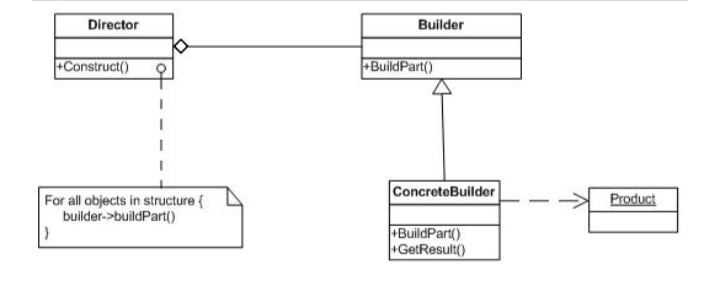
\includegraphics[scale=0.7]{./image/builder-pattern.jpg}
			\end{center}
		\end{figure}

        \subsection{Đặc điểm}
        \begin{itemize}
            \item[-]\subpara{Không cần truyền giá trị null cho các tham số không sử dụng}
            \item[-]\subpara{Kiểm soát tốt hơn quá trình xây dựng đối tượng}
            \item[-]\subpara{Có thể tạo đối tượng immutable}
        \end{itemize}

		\subsection{Mục Đích Sử Dụng}
		\begin{itemize}
			\item[-]\subpara{Tạo một đối tượng phức tạp: có nhiều thuộc tính (nhiều hơn 4) và một số bắt buộc, một số không bắt buộc}
			\item[-]\subpara{Tách rời quá trình xây dựng một đối tượng phức tạp từ các phần tạo nên đối tượng}
			\item[-]\subpara{Khi người dùng (client) mong đợi nhiều cách khác nhau cho đối tượng được xây dựng}
			\item[-]\subpara{Giảm bớt số lượng hàm constructor}
		\end{itemize}


		\subsection{Code khuôn mẫu}
		\begin{lstlisting}
package builder.pattern;
//Builder.java
public interface Builder {
    public void buildPartOne();
    public void buildPartTwo();
    public Product getProduct();
}

//Client.java
public class Client {
    public static void main(String[] args) {
        Director director = new Director(new ConcreteBuilder());
        director.makeProduct();

        Product product = director.getProduct();

        System.out.println("Product part: " + product.getPartOne());
        System.out.println("Product part: " + product.getPartTwo());
    }
}

//ConcreteBuilder.java
public class ConcreteBuilder implements Builder{
    private Product product;

    public ConcreteBuilder() {
        this.product = new Product();
    }

    @Override
    public void buildPartOne() {
        product.setPartOne("Part One");
    }

    @Override
    public void buildPartTwo() {
        product.setPartTwo("Part Two");
    }

    @Override
    public Product getProduct() {
        return product;
    }
}

//Director.java
public class Director {
    private Builder builder;

    public Director(Builder builder){
        this.builder = builder;
    }

    public void makeProduct(){
        builder.buildPartOne();
        builder.buildPartTwo();
    }

    public Product getProduct(){
        return builder.getProduct();
    }
}

//Product.java
public class Product {
    private String partOne;
    private String partTwo;

    public String getPartOne() {
        return partOne;
    }

    public void setPartOne(String partOne) {
        this.partOne = partOne;
    }

    public String getPartTwo() {
        return partTwo;
    }

    public void setPartTwo(String partTwo) {
        this.partTwo = partTwo;
    }
}
        \end{lstlisting}

		\subsection{Giải thích Design Pattern}
		\begin{itemize}
		    \item[-]\subpara{Giải thích theo mô hình}
		    \begin{itemize}
			    \item[+]\subpara{Product: đại diện cho đối tượng cần tạo, đối tượng này phức tạp, có nhiều thuộc tính.}
			    \item[+]\subpara{Builder: là abstract class hoặc interface khai báo phương thức tạo đối tượng.}
		    	\item[+]\subpara{ConcreteBuilder: kế thừa Builder và cài đặt chi tiết cách tạo ra đối tượng. Nó sẽ xác định và nắm giữ các instance mà nó tạo ra, đồng thời nó cũng cung cấp phương thức để trả các các thể hiện mà nó đã tạo ra trước đó. Hay nói cách khác là bản thiết kế từng bước của đối tượng Product}
			    \item[+]\subpara{Director/Client: là nơi sẽ gọi tới Builder để tạo ra đối tượng.}
			\end{itemize}
		    \item[-]\subpara{Giải thích theo code khuôn mấu}
		    \begin{itemize}
			    \item[+]\subpara{Khi chạy main của Client, đối tượng Director được khởi tạo, với đối đầu vào là 1 instance ConcreteBuilder được kế thừa từ Builder chứa thông tin từng bước}
			    \item[+]\subpara{Tiếp theo Client gọi hàm thực thi trong Director là hàm makeProduct chứa các bước trong interface builder từ đó gọi các hàm override bởi các hàm trong Builder ConcreteBuilder để thực hiện các bước dựng đối tượng}
			    \item[+]\subpara{Sau khi Director dựng xong đối tượng, Client lấy đối tượng Product về từ Director từ đó có thể sử dụng Product như bình thường}
	        \end{itemize}
		\end{itemize}

		\subsection{Ví Dụ Sử Dụng Trong Thực Tế}
\begin{itemize}
            \item[-]\subpara{Hệ thống quản lý tài khoản sử dụng builder parttern\\ https://github.com/blaplafla13th/design-partterns/tree/main/src/builder}
            \item[-]\subpara{Do tạo tài khoản hay đăng nhập, chúng ta cùng có hai bước là ghi nhận thông tin và xử lý thông tin như vậy chúng ta cần tạo một interface AccountBuilder với 2 step để xử lý với step 1 là điền thông tin, step 2 là xử lý dữ liệu và đọc ghi vào mảng cụ thể là accountArrayList ở Client.java. Tiếp theo tạo class builder của signIn và signUp để tạo form điền ở step1 và xử lý form ở step2.}
            \item[-]\subpara{Chúng ta tạo một AccountDirector để tạo đối tượng builder để chạy hai builder vừa tạo. Hàm dựng sẽ nhận bản thiết kế của class builder và thực hiện các bước. sau đó là hàm để return đối tượng}
            \item[-]\subpara{Về phía Client, ta cần tạo 1 arraylist để lưu tại khoản và hàm để gọi arraylist này. Trong main ta tạo biến current để lưu tài khoản hiện tại đóng vai trò quản lý phiên. Tạo một vòng lặp để lựa chọn đăng kí và đăng nhập và 2 director tương ứng với 2 lựa chọn đăng kí và đăng nhập. Tiếp theo chúng ta sẽ chạy hàm sign của Director để Directỏ chạy các bước như thiết kế.}
            \item[-]\subpara{Như vậy ta hoàn toàn có thể đọc sửa thông tin của account như ví dụ và lưu current vào mảng thay thế cho account hiện đăng nhập. Khi log out chúng ta đặt current = null để thoát phiên.}
        \end{itemize}
		\pagebreak

        \section{Factory}
        \subsection{Định Nghĩa Và Mô Hình Cấu Trúc}
        \begin{itemize}
            \item[-]\subpara{Factory sử dụng một interface hay một abstract class mà tất cả các lớp chúng ta cần khởi tạo đối tượng sẽ kế thừa. Factory sẽ khởi tạo một đối tượng mới mà không cần thiết phải chỉ ra chính xác class nào sẽ được khởi tạo}
            \item[-]\subpara{Mô hình:}
        \end{itemize}
		\begin{figure}[htp]
			\begin{center}
				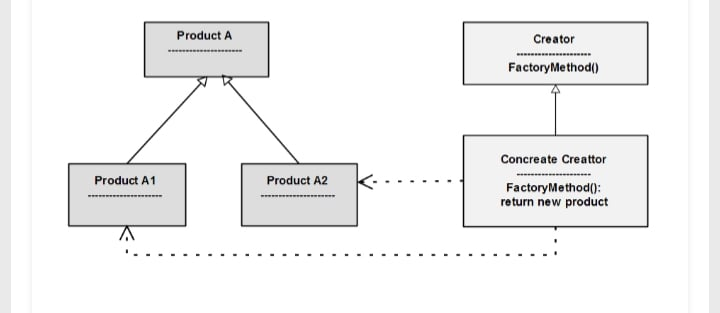
\includegraphics[scale=0.7]{./image/factory-pattern.jpg}
			\end{center}
		\end{figure}

        \subsection{Đặc điểm}
        \begin{itemize}
            \item[-]\subpara{Người dùng không biết logic thực sự được khởi tạo bên dưới phương thức factory}
            \item[-]\subpara{Cho phép các lớp con chọn kiểu đối tượng cần tạo}
            \item[-]\subpara{Code chỉ tương tác với interface hoặc lớp abstract}
            \item[-]\subpara{Dễ dàng quản lý file cycle của các đối tượng được tạo}
            \item[-]\subpara{Thống nhất về mặt naming convention}
        \end{itemize}

		\subsection{Mục Đích Sử Dụng}
		\begin{itemize}
			\item[-]\subpara{Tạo ra một cách mới trong việc khởi tạo đối tượng thông qua một interface chung}
			\item[-]\subpara{Che giấu đi xử lý logic của việc khởi tạo đối tượng}
			\item[-]\subpara{Giảm sự phụ thuộc giữa các module và tăng tính mở rộng code}
		\end{itemize}


		\subsection{Code khuôn mẫu}
		\begin{lstlisting}
package factory.pattern;
//Factory.java
public class Factory {
    public Product createProduct(String productType){
        switch (productType){
            case "a": return new ProductA();
            case "b": return new ProductB();
            ...
            default: return null;
        }
    };
}

//Product.java
public abstract class Product {
    ...
}

//ProductA.java
public class ProductA extends Product{
    public ProductA(){
        ...
    }
    ...
}

//ProductB, ... similar as class ProductA

//Client.java
public class Client{
    public static void main(String[] args){
        Factory factory = new Factory();
        Product product = factory.createProduct("a");
    }
}
        \end{lstlisting}

		\subsection{Giải thích Design Pattern}
		\begin{itemize}
		    \item[-]\subpara{Giải thích theo mô hình}
		    \begin{itemize}
			\item[+]\subpara{Super Class: môt super class (class A trong mô hình) trong Factory Pattern có thể là một interface, abstract class hay một class thông thường. các Sub Class (A1, A2,...) là các class kế thừa từ class A theo nhiệm vụ của nó}
			\item[+]\subpara{Class Concrete Creator hay Factory sẽ chịu tránh nhiệm khởi tạo các đối tượng sub class dựa theo tham số đầu vào và trả về cho Client. Thường thì class này là 1 Singleton. }
			\item[+]\subpara{Sau đó class Client hay Creator sẽ gọi đến Concrete Creator để lấy đối tượng mà chúng ta cần}
			\end{itemize}
		    \item[-]\subpara{Giải thích theo code khuôn mấu}
		    \begin{itemize}
			    \item[+]\subpara{Chúng ta có 1 superclass Product và các class con kế thừa class Product như ProductA, ProductB,...}
			    \item[+]\subpara{Class Factory có nhiệm vụ tạo đối tượng với 1 hàm createProduct với tham số là loại product. Trong hàm là 1 switch case để khi nhập 1 giá trị, hàm sẽ trở về 1 đối tượng mới tương ứng của Product. }
			    \item[+]\subpara{Về phía Client chúng ta tạo một instance của Factory rồi dùng hàm createProduct từ đối tượng factory để tạo ra đối tượng mình mong muốn}
			\end{itemize}
		\end{itemize}

		\subsection{Ví Dụ Sử Dụng Trong Thực Tế}
\begin{itemize}
            \item[-]\subpara{Hệ thống thanh toán đơn giản sử dụng factory parttern \\ https://github.com/blaplafla13th/design-partterns/tree/main/src/factory}
            \item[-]\subpara{chúng ta tạo 1 package paymentmethod để chứa interface PaymentMethod và các class implements từ PaymentMethod. Mõi class đều chứa tên phương thức, số tài khoản, tên người dùng và đoạn code ẩn để thanh toán}
            \item[-]\subpara{Tiếp theo tạo 1 class FactoryPaymentMethod chứa 1 hàm trả về đói tượng PaymentMethod với đối đầu vào là tên phương thức thanh toán và bên trong chứa 1 switch case các phương thức thanh toán và mỗi lựa chọn của switch case trả về 1 instance PaymentMethod tương ứng}
            \item[-]\subpara{Đối với Client ta dùng hàm listFile để gọi ra các phương thức thanh toán khả dụng. Khi người dùng nhập phương thức thanh toán, đối tượng factoryPaymentMethod được khởi tạo, chạy hàm getPaymentMethod để trả về phương thức thanh toán như yêu cầu từ đó người dùng có thể sử dụng các hàm trong phương thức thanh toán không biết được khởi tạo bên dưới phương thức factory }
            \item[-]\subpara{Khi cần thêm phương thức thanh toán, lập trình viên chỉ cần tạo 1 class mới trong package paymentmethod và thêm vào switch case của FactoryPaymentMethod}
        \end{itemize}
		\pagebreak

		\begin{center}
		    \hspace{0pt}
            \vfill
		    \fontsize{30}{20}\selectfont\part{Nhóm Cấu trúc - Structural Pattern}
		    \vfill
            \hspace{0pt}
	    \end{center}
	\pagebreak

		\section{Adapter}
        \subsection{Định Nghĩa Và Mô Hình Cấu Trúc}
        \begin{itemize}
            \item[-]\subpara{Adapter Pattern cho phép các interface không liên quan tới nhau có thể làm việc cùng nhau. Đối tượng giúp kết nối các interface gọi là Adapter}
            \item[-]\subpara{Adapter Pattern giữ vai trò trung gian giữa hai lớp, chuyển đổi interface của một hay nhiều lớp có sẵn thành một interface khác thích hợp cho lớp đang viết}
            \item[-]\subpara{Mô hình:}
        \end{itemize}
		\begin{figure}[htp]
			\begin{center}
				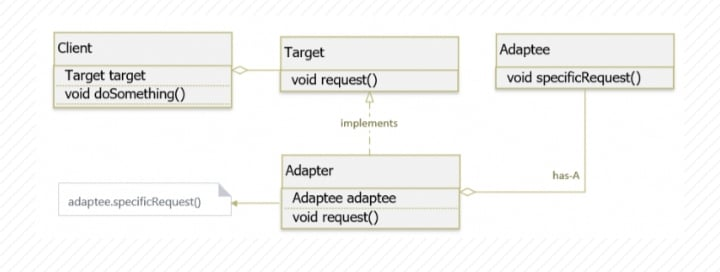
\includegraphics[scale=0.65]{./image/adapter-pattern.jpg}
			\end{center}
		\end{figure}

        \subsection{Đặc điểm}
        \begin{itemize}
            \item[-]\subpara{Phân tách việc chuyển đổi interface với business logic chính của chương trình}
            \item[-]\subpara{Có thể sử dụng adapter với các class con của adaptee}
            \item[-]\subpara{Làm việc với adapter class thay vì sửa đổi bên trong adaptee class đã có sẵn}
            \item[-]\subpara{Client tiếp cận thông qua interface thay vì implementation}
            \item[-]\subpara{Tăng chi phí và độ phức tạp của code}
        \end{itemize}

		\subsection{Mục Đích Sử Dụng}
		\begin{itemize}
			\item[-]\subpara{Chuyển đổi interface của một class thành interface mà client yêu cầu}
			\item[-]\subpara{Tạo ra những lớp có khả năng sử dụng lại, chúng phối hợp với các lớp không liên quan hay những lớp không thể đoán trước được và những lớp này không có interface tương thích}
			\item[-]\subpara{Khi muốn đảm bảo nguyên tắc Open/Close trong một ứng dụng}
		\end{itemize}


		\subsection{Code khuôn mẫu}
		\begin{lstlisting}
package adapter.pattern;
//Adaptee.java
public class Adaptee {
    public Adaptee(String name){

    }

    public void specificRequest() {
        System.out.println("Called specific request on Adaptee ");
    }
}

//Adapter.java
public class Adapter implements Target {
    private Adaptee adaptee;

    public Adapter(Adaptee adaptee){
        this.adaptee = adaptee;
    }

    @Override
    public void request() {
        adaptee.specificRequest();
    }
}

//Client.java
public class Client {
    public static void main(String[] args) {
        Target target = new Adapter(new Adaptee());
        target.request();
    }
}

//Target.java
public interface Target {
    public void request();
}
        \end{lstlisting}

		\subsection{Giải thích Design Pattern}
		\begin{itemize}
			\item[-]\subpara{Theo Mô hình}
			\begin{itemize}
			    \item[+]\subpara{Adaptee: là một class không tương thích, cần được tích hợp vào.}
			    \item[+]\subpara{Adapter: lớp tích hợp, giúp class không tương thích tích hợp được với interface đang làm việc. Thực hiện việc chuyển đổi interface cho Adaptee và kết nối Adaptee với Client.}
			    \item[+]\subpara{Target: một interface chứa các chức năng được sử dụng bởi Client (domain specific).}
			    \item[+]\subpara{Client: lớp sử dụng các đối tượng có interface Target.}
		\end{itemize}
			\item[-]\subpara{Theo code minh họa}
			\begin{itemize}
			    \item[+]\subpara{Class Adaptee có 1 phương thức cần}
			    \item[+]\subpara{Một interface Target sẽ chứa hàm request với mục đích để gọi hàm trong Adaptee}
			    \item[+]\subpara{Adapter sẽ implements interface Target, có một hàm dựng với tham số là instance của Adaptee. Hàm request của Adapter sẽ gọi đến hàm cần yêu cầu của Adaptee.}
			    \item[+]\subpara{Client: sẽ tạo instance của Adapter với đối số là một đối tượng adaptee mới. Như vậy ta có thể gọi hàm cần yêu cầu qua phương thức request trên target}
		    \end{itemize}
		\end{itemize}

		\subsection{Ví Dụ Sử Dụng Trong Thực Tế}
\begin{itemize}
            \item[-]\subpara{Dịch một chương trình đơn giản bằng adapter pattern\\https://github.com/blaplafla13th/design-partterns/tree/main/src/adapter}
            \item[-]\subpara{Ban đầu chúng ta có 2 file Program.java và Client.java. Program.java sử dụng hàm command và status để trả về các giá trị String rồi mới in chứ không in trực tiếp String bằng System.out.println.Class Program ở đây đóng vai trò của adaptee, giờ chúng ta sẽ viết 1 adapter và target}
            \item[-]\subpara{Ta tạo một interface Language chứa các hàm sẽ gọi của Program trong main làm target}
            \item[-]\subpara{Tạo một class implememt interface Language ở đây là class Vietnamese. Trong class ta sẽ dùng mảng String 2 chiều để lưu cặp giá trị String gồm từ chương trình trả về và từ chúng ta muốn dịch sang (mảng languagePack). Viết hàm translateMessage với tham số kiểu String để nhận giá trị chương trình trả về. Tạo 1 vòng for để tìm giá trị đó trong languagePack và trả về giá trị tương ứng của cặp. }
            \item[-]\subpara{Trong các hàm implement từ Language chúng ta sẽ trả về giá trị mà translateMessage trả về từ tham số tương ứng với đối số truyền vào là kết qủa của hàm tương ứng bên file Program.java\\ Ví dụ như hàm run trong Vietnamese sẽ lấy tham số truyền vào giống hàm run ở Program trả về là translateMessage với đối số truyền vào là kết quả trả về của hàm run bên Program. }
            \item[-]\subpara{Đối với Client.java, chúng ta tạo một instance kiểu Language của class Vietnamese với đối số truyền vào là Program và thay vì gọi đến hàm trong instance Program thì chúng ta gọi đến instance của Language. Hay đơn giản hơn thay vì chúng ta sửa dòng tạo đối tượng Program thành tạo đối tượng kiểu  Language của class Vietnamese, đối số là đối tượng Program mới, giữ nguyên tên biến là ta đã dịch thành công chương trình}
            \item[-]\subpara{Trong thực tế cách này được dùng để dịch các chương trình sử dụng bộ các keyword:value để in thông tin, keyword:value thường được lưu ra file riêng, sẽ có hàm đọc file này để ghi vào mảng languagePack ở trên, cách này không dịch được các thông tin cứng được in trực tiếp mà không có trong bộ keyword:value}
        \end{itemize}
		\pagebreak

		\section{Bridge}
        \subsection{Định Nghĩa Và Mô Hình Cấu Trúc}
        \begin{itemize}
            \item[-]\subpara{Bridge Pattern tách tính trừu tượng (abstraction) ra khỏi tính hiện thực (implementation) của nó. Từ đó, có thể dễ dàng chỉnh sửa hoặc thay thế mà không làm ảnh hưởng đến những nơi có sử dụng lớp ban đầu}
            \item[-]\subpara{Mô hình:}
        \end{itemize}
		\begin{figure}[htp]
			\begin{center}
				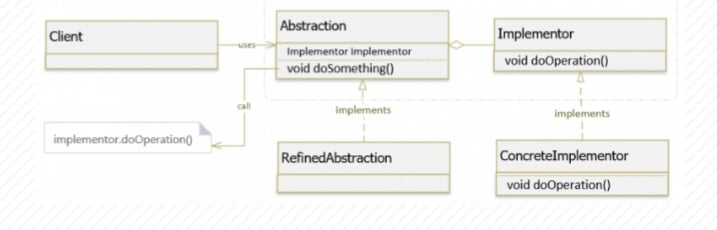
\includegraphics[scale=0.65]{./image/bridge-pattern.jpg}
			\end{center}
		\end{figure}

        \subsection{Đặc điểm}
        \begin{itemize}
            \item[-]\subpara{Giảm sự phụ thuộc giữa abstraction và implementation}
            \item[-]\subpara{abstraction và implementation thay vì liên hệ bằng quan hệ kế thừa thì sẽ liên hệ với nhau thông qua object composition}
            \item[-]\subpara{Cho phép ẩn các chi tiết implement từ client}
            \item[-]\subpara{Dễ bảo trì và mở rộng về sau}
        \end{itemize}

		\subsection{Mục Đích Sử Dụng}
		\begin{itemize}
			\item[-]\subpara{Tách ràng buộc giữa abstraction và implementation để có thể dễ dàng mở rộng độc lập nhau}
			\item[-]\subpara{Thay đổi được thực thi trong implement mà không ảnh hưởng đến phía client}
		\end{itemize}


		\subsection{Code khuôn mẫu}
		\begin{lstlisting}
package bridge.pattern;
//Abtraction.java
public interface Abstraction {
	void operacion();
}

//Client.java
public class Client {
	public static void main(String[] args) {
        Abstraction[] abstracciones = new Abstraction[2];
        abstracciones[0] = new RefinedAbstraction(new ImplementorA());
        abstracciones[1] = new RefinedAbstraction(new ImplementorB());

        for(Abstraction abstraccion:abstracciones) {
            abstraccion.operacion();
        }
    }
}

//ConcreteImplementor.java
public class ConcreteImplementor implements Implementor{
	public void operacion() {
        System.out.println("This is implementacion");
    }
}

//Implementor.java
public interface Implementor {
	void operacion();
}

//RefinedAbstraction.java
public class RefinedAbstraction implements Abstraction{
    private Implementor implementador;

    public RefinedAbstraction(Implementor implementador){
        this.implementador = implementador;
    }

    public void operacion(){
        implementador.operacion();
    }
}
        \end{lstlisting}

		\subsection{Giải thích Design Pattern}
		\begin{itemize}
			\item[-]\subpara{Theo Mô hình ct}
			\item[-]\subpara{Theo code minh họa}
		\end{itemize}

		\subsection{Ví Dụ Sử Dụng Trong Thực Tế}
\begin{itemize}
            \item[-]\subpara{}<ý 1>
            \item[-]\subpara{}<ý 2>
        \end{itemize}
		\pagebreak

        \section{Decorator}
        \subsection{Định Nghĩa Và Mô Hình Cấu Trúc}
        \begin{itemize}
            \item[-]\subpara{Decorator Pattern thay đổi một instance riêng lẻ của một class bằng cách tạo một class decorator bao bọc class gốc. Như vậy, việc thay đổi hoặc thêm chức năng của object decorator không ảnh hưởng đến cấu trúc hoặc chức năng của object ban đầu}
            \item[-]\subpara{Mô hình:}
        \end{itemize}
		\begin{figure}[htp]
			\begin{center}
				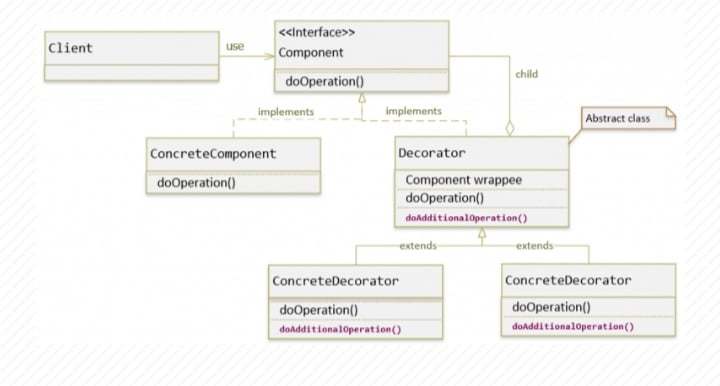
\includegraphics[scale=0.65]{./image/decorator-pattern.jpg}
			\end{center}
		\end{figure}

        \subsection{Đặc điểm}
        \begin{itemize}
            \item[-]\subpara{Có thể bổ sung những chức năng mới cho object}
            \item[-]\subpara{Object gốc không thay đổi và không biết gì về những thứ được bổ sung cho nó}
            \item[-]\subpara{Được thực hiện trong thời gian chạy và chỉ áp dụng cho một cá thể}
            \item[-]\subpara{Không cần phải xây dựng class khổng lồ với mọi thứ bên trong}
            \item[-]\subpara{Các object decorator độc lập nhau và có thể tổ hợp với nhau}
        \end{itemize}

		\subsection{Mục Đích Sử Dụng}
		\begin{itemize}
			\item[-]\subpara{Thêm tính năng mới cho đối tượng mà không ảnh hưởng đến các đối tượng này}
			\item[-]\subpara{Trong các trường hợp mà việc sử dụng kế thừa sẽ mất nhiều công sức trong việc viết code hoặc không thể mở rộng đối tượng bằng thừa kế}
		\end{itemize}


		\subsection{Code khuôn mẫu}
		\begin{lstlisting}
package decorator.pattern;
//Client.java
public class Client {
    public static void main(String[] args) {
        Component component = new ConcreteDecoratorOne(new ConcreteComponent());
        component.doOperation();
        System.out.println("Adding concrete component two...");
        component = new ConcreteDecoratorOne(new ConcreteDecoratorTwo(new ConcreteComponent()));
        component.doOperation();
    }
}

//Component.java
public interface Component {
    public void doOperation();
}

//ConcreteComponent.java
public class ConcreteComponent implements Component {
    @Override
    public void doOperation() {
        System.out.println("Concrete Component doing operation");
    }
}

//ConcreteDecorator.java
public class ConcreteDecorator extends Decorator {
    public ConcreteDecorator(Component component) {
        super(component);
    }

    @Override
    public void doOperation() {
        super.doOperation();
        doAdditionalOperation();
    }

    public void doAdditionalOperation() {
        System.out.println("Doing additional operation concrete decorator.");
    }
}

//Decorator.java
public abstract class Decorator implements Component {
    protected Component component;

    public Decorator(Component component){
        this.component = component;
    }

    @Override
    public void doOperation() {
        component.doOperation();
    }
}
        \end{lstlisting}

		\subsection{Giải thích Design Pattern}
		\begin{itemize}
			\item[-]\subpara{Theo Mô hình ct}
			\item[-]\subpara{Theo code minh họa}
		\end{itemize}

		\subsection{Ví Dụ Sử Dụng Trong Thực Tế}
\begin{itemize}
            \item[-]\subpara{}<ý 1>
            \item[-]\subpara{}<ý 2>
        \end{itemize}
		\pagebreak

		\begin{center}
		    \hspace{0pt}
		    \vfill
		    \fontsize{30}{20}\selectfont\part{Nhóm hành vi - Behavioral Pattern}
	        \vfill
            \hspace{0pt}
	    \end{center}
	\pagebreak

		\section{Observer}
        \subsection{Định Nghĩa Và Mô Hình Cấu Trúc}
\begin{itemize}
            \item[-]\subpara{}<ý 1>
            \item[-]\subpara{}<ý 2>
        \end{itemize}

        \subsection{Đặc điểm}
        \begin{itemize}
            \item[-]\subpara{}<đặc điểm 1>
            \item[-]\subpara{}<đặc điểm 2>
        \end{itemize}

		\subsection{Mục Đích Sử Dụng}
		\begin{itemize}
			\item[-]\subpara{}<mục đích 1>
			\item[-]\subpara{}<mục đích 2>
		\end{itemize}

		\subsection{Code khuôn mẫu}
		\begin{lstlisting}

        \end{lstlisting}

		\subsection{Giải thích Design Pattern}
		\begin{itemize}
			\item[-]\subpara{Theo Mô hình ct}
			\item[-]\subpara{Theo code minh họa}
		\end{itemize}

		\subsection{Ví Dụ Sử Dụng Trong Thực Tế}
\begin{itemize}
            \item[-]\subpara{}<ý 1>
            \item[-]\subpara{}<ý 2>
        \end{itemize}
		\pagebreak

		\section{Iterator}
        \subsection{Định Nghĩa Và Mô Hình Cấu Trúc}
\begin{itemize}
            \item[-]\subpara{}<ý 1>
            \item[-]\subpara{}<ý 2>
        \end{itemize}

        \subsection{Đặc điểm}
        \begin{itemize}
            \item[-]\subpara{}<đặc điểm 1>
            \item[-]\subpara{}<đặc điểm 2>
        \end{itemize}

		\subsection{Mục Đích Sử Dụng}
		\begin{itemize}
			\item[-]\subpara{}<mục đích 1>
			\item[-]\subpara{}<mục đích 2>
		\end{itemize}

		\subsection{Code khuôn mẫu}
		\begin{lstlisting}

        \end{lstlisting}

		\subsection{Giải thích Design Pattern}
		\begin{itemize}
			\item[-]\subpara{Theo Mô hình ct}
			\item[-]\subpara{Theo code minh họa}
		\end{itemize}

		\subsection{Ví Dụ Sử Dụng Trong Thực Tế}
\begin{itemize}
            \item[-]\subpara{}<ý 1>
            \item[-]\subpara{}<ý 2>
        \end{itemize}
		\pagebreak

        \section{Command}
        \subsection{Định Nghĩa Và Mô Hình Cấu Trúc}
\begin{itemize}
            \item[-]\subpara{}<ý 1>
            \item[-]\subpara{}<ý 2>
        \end{itemize}

        \subsection{Đặc điểm}
        \begin{itemize}
            \item[-]\subpara{}<đặc điểm 1>
            \item[-]\subpara{}<đặc điểm 2>
        \end{itemize}

		\subsection{Mục Đích Sử Dụng}
		\begin{itemize}
			\item[-]\subpara{}<mục đích 1>
			\item[-]\subpara{}<mục đích 2>
		\end{itemize}

		\subsection{Code khuôn mẫu}
		\begin{lstlisting}

        \end{lstlisting}

		\subsection{Giải thích Design Pattern}
		\begin{itemize}
			\item[-]\subpara{Theo Mô hình ct}
			\item[-]\subpara{Theo code minh họa}
		\end{itemize}

		\subsection{Ví Dụ Sử Dụng Trong Thực Tế}
\begin{itemize}
            \item[-]\subpara{}<ý 1>
            \item[-]\subpara{}<ý 2>
        \end{itemize}
		\pagebreak

		\section{Strategy}

        \subsection{Định Nghĩa Và Mô Hình Cấu Trúc}
\begin{itemize}
            \item[-]\subpara{}<ý 1>
            \item[-]\subpara{}<ý 2>
        \end{itemize}

        \subsection{Đặc điểm}
        \begin{itemize}
            \item[-]\subpara{}<đặc điểm 1>
            \item[-]\subpara{}<đặc điểm 2>
        \end{itemize}

		\subsection{Mục Đích Sử Dụng}
		\begin{itemize}
			\item[-]\subpara{}<mục đích 1>
			\item[-]\subpara{}<mục đích 2>
		\end{itemize}

		\subsection{Code khuôn mẫu}
		\begin{lstlisting}

        \end{lstlisting}

		\subsection{Giải thích Design Pattern}
		\begin{itemize}
			\item[-]\subpara{Theo Mô hình ct}
			\item[-]\subpara{Theo code minh họa}
		\end{itemize}

		\subsection{Ví Dụ Sử Dụng Trong Thực Tế}
\begin{itemize}
            \item[-]\subpara{}<ý 1>
            \item[-]\subpara{}<ý 2>
        \end{itemize}
		\pagebreak

		\part{TÀI LIỆU THAM KHẢO}
				\begin{itemize}
			\item[1]\subpara{. Slides Bài giảng}
			\item[2]\subpara{. Head First Design Patterns}
			\item[3]\subpara{. https://sourcemaking.com/design-patterns}
			\item[4]\subpara{. https://github.com/LuisBurgs/design-patterns}
			\item[5]\subpara{. https://gpcoder.com/4164-gioi-thieu-design-patterns/}
        \end{itemize}
\end{document}
